\chapter{Grenz- und Richtwerte für den Fahrkomfort}\label{app:Tabelle}
	\begin{table}[h]
		\caption{Zusammenfassung der Grenz- und Richtwerte für die Längsdynamik}
		\label{tab:Komfortwerte_längs}
		\begin{tabular}[h]{|p{3.3cm}|p{9cm}|p{2cm}|p{1cm}|}\hline
			\textbf{Größe} & \textbf{Beschreibung} & \textbf{Wert} & \textbf{Quelle} \\ \hline
			\rule[2mm]{0mm}{3mm}Längsbeschleunigung & Maximalwert für \gls{FSRA} für $v>\valunit{20}{km/h}$ & \valunit{2}{m/s^2} & \cite{Winner.2012} \\
			\cline{2-4}\rule[2mm]{0mm}{3mm}
			& Maximalwert für \gls{FSRA} für $v<\valunit{5}{km/h}$ & \valunit{4}{m/s^2} & \cite{Winner.2012} \\
			\cline{2-4}\rule[2mm]{0mm}{3mm}
			& Schwellwert zur Unterscheidung zwischen komfortabler und unkomfortabler Fahrt & \valunit{2}{m/s^2} & \cite{Liu.2005} \\
			\cline{2-4}\rule[2mm]{0mm}{3mm}
			& Mittlere Beschleunigung eines undynamischen Fahrstils auf Landstraßen & \valunit{1}{m/s^2} & \cite{Radke.2013} \\
			\cline{2-4}\rule[2mm]{0mm}{3mm}
			& Höchstwert des 90. Perzentils von Anfahrbeschleunigungen bei Geradeausfahrt & \valunit{2{,}56}{m/s^2} & \cite{Krause.2002} \\
			\cline{2-4}\rule[2mm]{0mm}{3mm}
			& Höchstwert des 90. Perzentils von Anfahrbeschleunigungen beim Rechtsabbiegen & \valunit{2{,}2}{m/s^2} & \cite{Krause.2002} \\	\cline{2-4}\rule[2mm]{0mm}{3mm}
			& Wert des 90. Perzentils von Beschleunigungen bei Alltagsfahrten & \valunit{2{,}6}{m/s^2} & \cite{Hugemann.2003} \\
			\cline{2-4}\rule[2mm]{0mm}{3mm}
			& Maximalwert der Beschleunigung bei hohem Komfortniveau & \valunit{2}{m/s^2} & \cite{Schwab.2019} \\
			\hline
			\rule[2mm]{0mm}{3mm}Längsverzögerung & Maximalwert für \gls{FSRA} für $v>\valunit{20}{km/h}$ & \valunit{-3{,}5}{m/s^2} & \cite{Winner.2012} \\
			\cline{2-4}\rule[2mm]{0mm}{3mm}
			& Maximalwert für \gls{FSRA} für $v<\valunit{5}{km/h}$ & \valunit{-5}{m/s^2} & \cite{Winner.2012} \\
			\cline{2-4}\rule[2mm]{0mm}{3mm}
			& Wert des 90. Perzentils von Verzögerungen bei Alltagsfahrten & \valunit{-3{,}3}{m/s^2} & \cite{Hugemann.2003} \\
			\cline{2-4}\rule[2mm]{0mm}{3mm}
			& Maximalwert der Verzögerung bei hohem Komfortniveau & \valunit{-2{,}5}{m/s^2} & \cite{Schwab.2019} \\
			\hline
			\rule[2mm]{0mm}{3mm}Längsruck & Maximalwert für \gls{FSRA} für $v>\valunit{20}{km/h}$ & $\pm$\valunit{2{,}5}{m/s^3} & \cite{Winner.2012} \\
			\cline{2-4}\rule[2mm]{0mm}{3mm}
			& Maximalwert für \gls{FSRA} für $v<\valunit{5}{km/h}$ & $\pm$\valunit{5}{m/s^3} & \cite{Winner.2012} \\
			\cline{2-4}\rule[2mm]{0mm}{3mm}
			& Typischer Grenzwert zur Wahrung von Passagierkomfort& $\pm$\valunit{2}{m/s^3} & \cite{CanudasdeWit.2005} \\
			\hline
		\end{tabular}
	\end{table}

	\begin{table}[h]
		\caption{Zusammenfassung der Grenz- und Richtwerte für die Querdynamik}
		\label{tab:Komfortwerte_quer}
		\begin{tabular}[h]{|p{3.3cm}|p{9cm}|p{2cm}|p{1cm}|}\hline
			\textbf{Größe} & \textbf{Beschreibung} & \textbf{Wert} & \textbf{Quelle} \\ \hline
			\rule[2mm]{0mm}{3mm}Querbeschleunigung & Maximalwert für \gls{LKS} für $\valunit{60}{km/h}<v<\valunit{180}{km/h}$ & \valunit{2}{m/s^2} & \cite{Gayko.2012} \\
			\cline{2-4}\rule[2mm]{0mm}{3mm}
			& Mittlere Beschleunigung eines undynamischen Fahrstils auf Landstraßen & \valunit{2{,}5}{m/s^2} & \cite{Radke.2013} \\
			\cline{2-4}\rule[2mm]{0mm}{3mm}
			& Maximalwert der Beschleunigung bei hohem Komfortniveau & \valunit{1{,}8}{m/s^2} & \cite{Schwab.2019} \\
			\cline{2-4}\rule[2mm]{0mm}{3mm}
			& Maximalwert der Beschleunigung eines defensiven Fahrstils & \valunit{2{,}9}{m/s^2} & \cite{Schwab.2019} \\
			\cline{2-4}\rule[2mm]{0mm}{3mm}
			& Höchstwert typischer Beschleunigungen von \GenderPl{Normalfahrer} in der Stadt & ca. \valunit{3{,}2}{m/s^2} & \cite{Dragon.2008} \\
			\cline{2-4}\rule[2mm]{0mm}{3mm}
			& Höchstwert typischer Beschleunigungen von \GenderPl{Normalfahrer} auf Landstraßen & ca. \valunit{4{,}1}{m/s^2} & \cite{Dragon.2008} \\
			\cline{2-4}\rule[2mm]{0mm}{3mm}
			& Höchstwert typischer Beschleunigungen von \GenderPl{Normalfahrer} auf Autobahnen & ca. \valunit{2}{m/s^2} & \cite{Dragon.2008} \\
			\cline{2-4}\rule[2mm]{0mm}{3mm}
			& Selbstgewählte Beschleunigungen bei Fahrstreifenwechseln & $0{,}74$ bis $\valunit{1{,}01}{m/s^2}$ & \cite{Lange.2014} \\
			\cline{2-4}\rule[2mm]{0mm}{3mm}
			& Selbstgewählte Beschleunigungen bei Fahrstreifenwechseln mit geringer Querdynamik & \valunit{1{,}1}{m/s^2} & \cite{WorkshopAssistenzsystemeFestner.2017} \\
			\hline
			Querruck & Selbstgewählter Ruck bei Fahrstreifenwechseln mit geringer Querdynamik & $\pm$\valunit{1{,}8}{m/s^3} & \cite{WorkshopAssistenzsystemeFestner.2017} \\
			\hline
		\end{tabular}
	\end{table}

\chapter{\texttt{bvp4c}-Solver}\label{app:bvp4c}
Die Eigenschaft, dass sich Kollokationsverfahren mit stückweise definierten Polynomen durch \gls{RKV} ausdrücken lassen, machten sich Kierzenka und Shampine bei der Entwicklung des \texttt{bvp4c}-Solvers zu Nutze \cite{Kierzenka.2001}. Auf den $N$ Subintervallen wird die Lösung des \gls{ZPR} unter Verwendung der Lobatto-Kollokation (siehe \ref{subsubsec:Kollokationsverfahren_indirekt}) durch kubische Polynome approximiert, die neben den Randbedingungen \eqref{eq:Anfangswerte}--\eqref{eq:Transversalitaet} noch die Kollokationsbedingungen \eqref{eq:Kollokationsbedingung} an den Kollokationsstellen und die Stetigkeitsbedingungen \eqref{eq:Stetigkeitsbedingung} an den Intervallgrenzen erfüllen \cite{Kierzenka.2001}. Mit \eqref{eq:Kollokationsbedingung} und \eqref{eq:Stetigkeitsbedingung} erhält man so auf dem Gesamtintervall glatte Funktionen, die die Eigenschaft $S(t) \in \mathcal{C}^1[t_0, t_f]$ besitzen \cite{Kierzenka.2001}. Die Verwendung der Lobatto-Kollokation mit $k=3$ führt dabei auf ein 3-stufiges \gls{RKV}, welches mit der Schrittweite $h=t_{i+1}-t_i$ und  
\begin{align}
k_1 &= f(t_i,x_i) \\
k_2 &= f(t_{i+\frac{1}{2}},x_i+\frac{h}{24}(5k_1+8k_2-k_3)) \\
k_3 &= f(t_{i+1},x_i+\frac{h}{6}(k_1+4k_2+k_3)) = f(t_{i+1},x_{i+1})
\end{align}
auf das als \textit{Simpsonregel} bekannte implizite \gls{RKV}
\begin{equation}
x_{i+1} - x_i = \frac{h}{6}(k_1+4k_2+k_3)
\end{equation} 
führt \cite{Cash.1980}, dessen Fehlerordnung mit $\mathcal{O}(h^4)$ angegeben werden kann \cite{Kierzenka.2001}. Mithilfe dieser Formulierung lässt sich eine hohe Lösungsgenauigkeit erzielen. Eine residuengesteuerte Gitteranpassung, die den Fehler der Schätzung auf jedem Subintervall auswertet, trägt dazu bei, dass auch bei schlechter Gitterwahl akkurate Lösungen gefunden werden können \cite{Kierzenka.2001}. Zusätzlich lassen sich unbekannte Parameter (z.B. ein freier Endzeitpunkt) und allgemeine Randbedingungen berücksichtigen, wodurch die Funktion flexibel für verschiedene Problemstellungen angewendet werden kann. Darüber hinaus können auch interne \gls{GNB} berücksichtigt und so neben \gls{ZPR} auch allgemeine \gls{MPR} gelöst werden. Damit stellt dieser Solver eine effiziente und genaue Lösungsmethode für eine breite Klasse von Randwertproblemen dar. Eine weitere nützliche Eigenschaft des Solvers ist die Option, das Ergebnis eines Optimierungsdurchlaufs als Initialisierung für einen erneuten Durchlauf zu verwenden. Diese als \textit{Continuation} bezeichnete Vorgehensweise bietet die Möglichkeit, ungenaue Lösungen mithilfe mehrfacher Neuinitialisierungen zu verbessern und so eine deutlich höhere Ergebnisgüte zu erzielen \cite{Kierzenka.2001}. Eine Möglichkeit Continuation effektiv auszunutzen liegt darin, zunächst mithilfe einer zufälligen Initialisierung der Zustände eine Lösung zu erhalten. Diese ist möglicherweise noch zu ungenau, weshalb diese Lösung als Startwert für eine erneute Lösung des Randwertproblems genutzt werden kann, die dann eine höhere Genauigkeit erreicht. Dadurch kann das Problem, dass geeignete Startverläufe für die adjungierten Zustände geschätzt werden müssen, umgangen werden, da es ausreichend ist, einmal eine grobe Lösung zu erhalten und ausgehend von dieser die tatsächliche Lösung zu verfeinern. Eine weitere Möglichkeit zur Nutzung von Continuation besteht darin, die Lösung bei einer bestimmten Parametrierung des Problems zu bestimmen, indem man sich dieser Parametrierung sukzessive annähert. Die Lösung einer bestimmten Wunschparametrierung lässt sich so ausgehend von der Lösung bei einer Parametrierung, die noch weit von der Wunschparametrierung entfernt ist, durch stetiges Annähern an die Wunschparametrierung und Reinitialisieren berechnen.

\chapter{Abbildung zur Stellgröße beim Heranfahren an eine Ampel bei bekannter Rotphase}\label{app:Stellgr}
\begin{figure}[h] 
	\centering
	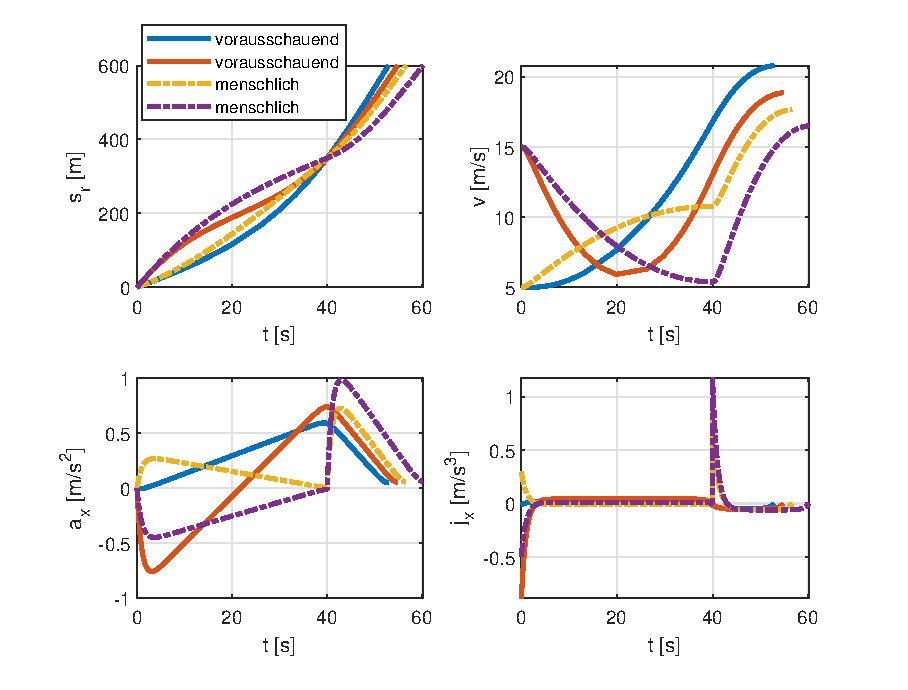
\includegraphics[width=\linewidth]{./Bilder/Ergebnisse/Geradeausfahrt/Ampel/v_5_v_15/svaj.eps}
	\caption{Lösungstrajektorien der Fahrzeugzustände und der Stellgröße beim Zufahren auf eine Ampel mit bekannter Rotphase. Darstellung der Ergebnisse für vorausschauende und menschliche (weniger vorausschauend) Planung bei unterschiedlichen Startgeschwindigkeiten. Ergänzung zu Abbildung \ref{fig:svaj_zoomj}.}
	\label{fig:svaj}
\end{figure} 